\subsubsection{Extension 1}
\begin{namedframe}{Diameters and right angles}
	\begin{example}
		Show that if the chord $AB$ is a diameter then $\angle ACB = \SI{90}{\degree}$.

		In other words, show that the angle subtended by a diameter is a right angle.
	\end{example}
	\centering
	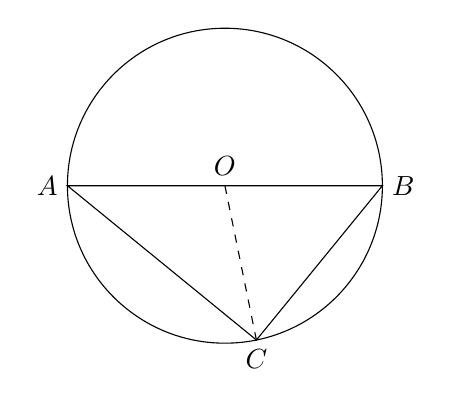
\begin{tikzpicture}[scale=0.4]
		\coordinate [label=above:$O$](O) at (0,0);
		\coordinate [label=left:$A$](A) at (-5,0);
		\coordinate [label=right:$B$](B) at (5,0);
		\coordinate [label=below:$C$](C) at (1,-4.89897948557);

		\draw (O) circle (5);
		\draw (A) -- (O) -- (B) -- (C) -- cycle;
		\draw [dashed] (O) -- (C);
	\end{tikzpicture}
\end{namedframe}
\begin{namedframe}{Extension 1 proof}
	\footnotesize
	\begin{proof}[Proof that $\angle ACB = \SI{90}{\degree}$.]
		\begin{wrapfigure}[7]{r}{0pt}
			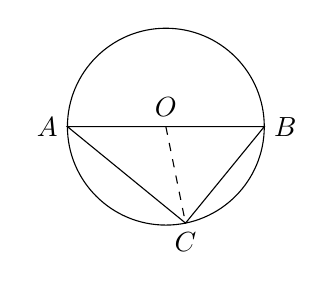
\begin{tikzpicture}[scale=0.25]
				\coordinate [label=above:$O$](O) at (0,0);
				\coordinate [label=left:$A$](A) at (-5,0);
				\coordinate [label=right:$B$](B) at (5,0);
				\coordinate [label=below:$C$](C) at (1,-4.89897948557);

				\draw (O) circle (5);
				\draw (A) -- (O) -- (B) -- (C) -- cycle;
				\draw [dashed] (O) -- (C);
			\end{tikzpicture}
		\end{wrapfigure}
		We know that $\angle ACO = \angle CAO$.
		So:
		\begin{equation}\label{eq:ex1:1}
			2\angle ACO + \angle AOC = \SI{180}{\degree}
		\end{equation}
		\pause
		Similarly:
		\begin{equation}\label{eq:ex1:2}
			2\angle BCO + \angle BOC = \SI{180}{\degree}
		\end{equation}
		\pause
		We also know that $\angle AOC = \SI{180}{\degree} - \angle BOC$.
		\sep[0pt]
		We substitute this into \eqref{eq:ex1:1} to get $2\angle ACO = \angle BOC$.
		\sep[0pt]
		We substitute this into \eqref{eq:ex1:2} to get:
		\begin{align*}
			2\angle BCO + 2\angle ACO &= \SI{180}{\degree}\\
			\angle BCO + \angle ACO &= \SI{90}{\degree}
		\end{align*}
		\pause
		Since $\angle BCO + \angle ACO = \angle ACB$, we arrive at:
		\pause
		\[\angle ACB = \SI{90}{\degree} \qedhere\]
	\end{proof}
\end{namedframe}
